\chapter{The results, figure by figure}

Each section shows one figure from the paper, explains every part of it, gives the key numbers, and ends with the one sentence you would say about it.

\section{How to read the bar charts}

Most figures are \term{grouped bar charts}:
\begin{itemize}
\item The horizontal axis lists groups (sibling types, models, or window situations).
\item Within each group, one bar per condition. Colours are the same in every figure: \textcolor{ancblue}{\textbf{blue}} ancestor-only, \textcolor{sibor}{\textbf{orange}} full tree, \textbf{green} sliding window.
\item The height of a bar is a rate or an average.
\item The small black whisker on each bar is its 95\% confidence interval (Chapter 8).
\item The number above each bar is the value, rounded.
\end{itemize}
If two whiskers do not overlap, the difference is clearly larger than chance variation.

\section{Token savings (paper Fig.~2)}

\begin{center}
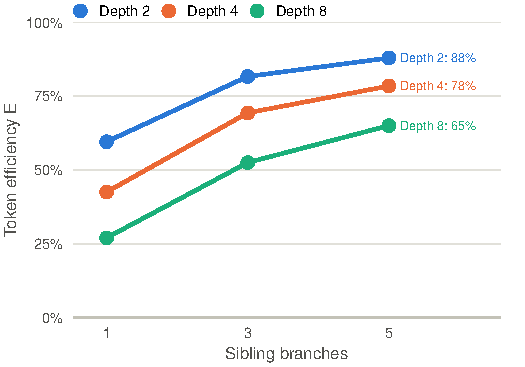
\includegraphics[width=0.75\textwidth]{fig3_efficiency.pdf}
\end{center}

\textbf{What it shows.} Token efficiency $E$ (how much of the full tree ancestor-only leaves out) on the vertical axis, against the number of sibling branches on the horizontal axis. One line per active-path depth. Each point averages 80 scenarios. The whiskers are there but tiny, because $E$ hardly varies within a cell.

\textbf{How to read it.} Higher is a bigger saving. Lines go up to the right: more siblings, more saved. Lines are lower for greater depth: a longer active path means ancestor-only itself is bigger, so the saving is a smaller share.

\begin{example}
Average saving across all scenarios: 62.7\%. Ancestor-only prompts averaged 474 reference tokens against 1,375 for the full tree. Smallest saving: 27.0\% (depth 8, one sibling). Largest: 87.9\% (depth 2, five siblings). The measured saving equalled the siblings' token share in every scenario, as Proposition 1 predicts.
\end{example}

\textbf{In one sentence:} ancestor-only always saves exactly the share of the conversation taken up by side branches, which was 63\% on average and up to 88\%.

\section{Leakage by sibling type (paper Fig.~3)}

\begin{center}
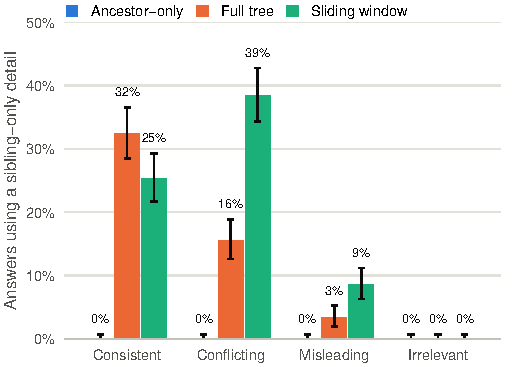
\includegraphics[width=0.75\textwidth]{fig1_leakage.pdf}
\end{center}

\textbf{What it shows.} The share of answers that \emph{used} a detail found only in an abandoned branch (judge-confirmed), for each sibling type and condition. About 540 answers per bar, all three models pooled.

\textbf{How to read it.} Every blue bar is zero: ancestor-only never leaked. Look at orange against green within each group to compare the full tree with the window.

\begin{example}
\begin{center}
\small
\begin{tabular}{@{}lrrr@{}}
\toprule
Sibling type & Ancestor & Full tree & Window \\
\midrule
Consistent & 0\% & 32.4\% & 25.4\% \\
Conflicting & 0\% & 15.6\% & 38.5\% \\
Misleading & 0\% & 3.3\% & 8.5\% \\
Irrelevant & 0\% & 0\% & 0\% \\
\bottomrule
\end{tabular}
\end{center}
\end{example}

\textbf{What the numbers mean.}
\begin{itemize}
\item \textbf{Consistent} siblings leaked most in the full tree. The extra detail is true and fits, so models happily include it (for example, using the column name \texttt{zr\_9fg}).
\item \textbf{Conflicting} siblings leaked much more in the window (38.5\%) than in the full tree (15.6\%). In the full tree, the model can see the real decision and the alternatives side by side and usually picks the real one. In the window, the real decision has often been pushed out, so the alternative is the only answer left. Among window prompts that contained a conflicting value, the model adopted it 86.9\% of the time, against 7.5\% in the full tree.
\item \textbf{Misleading} siblings rarely leaked. Models usually recognised the false claim and rejected it.
\item \textbf{Irrelevant} siblings never leaked. A wiki name or a lunch order number has no reason to appear in an answer about caching.
\end{itemize}

\textbf{The regression's view.} The window leaked $+25.5$ points more than the full tree for conflicting siblings (interval $+20.2$ to $+30.7$), $+2.7$ more for misleading ($+1.2$ to $+4.2$), and $8.2$ points \emph{less} for consistent ($-13.6$ to $-2.8$), all significant after Holm correction. Other factors: leakage rose with depth (OR 7.96 for depth 8 against depth 2) and with late siblings (OR 2.70), and GPT and Mistral leaked much less than Gemini (OR 0.12 and 0.13).

\begin{ask}
\textbf{``Why did deeper conversations leak more?''}\par
A deeper active path means a bigger ancestor-only size, so the window gets a bigger budget and has more room for sibling messages, and the full tree is longer too. The effect is about the baselines; ancestor-only stays at zero at every depth.
\end{ask}

\textbf{In one sentence:} ancestor-only never leaked; the full tree mostly leaked harmless true details, while the window, having lost the real decision, adopted conflicting alternatives in over a third of answers.

\section{Mentioned is not used (paper Fig.~4)}

\begin{center}
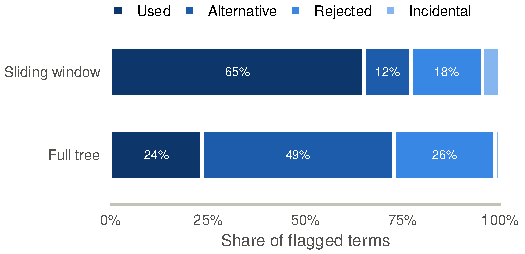
\includegraphics[width=0.75\textwidth]{fig2_term_usage.pdf}
\end{center}

\textbf{What it shows.} Every sibling term the string matcher found in an answer, split by how the leak judge labelled it. Each bar adds up to 100\%. The full-tree bar covers 1,455 terms; the window bar covers 837.

\textbf{How to read it.} The darkest segment (``Used'') is real leakage. The other segments are mentions that do not adopt the term.

\begin{example}
Full tree: used 23.5\%, alternative 49.2\%, rejected 26.0\%, incidental 1.3\%. Window: used 65.0\%, alternative 12.1\%, rejected 18.4\%, incidental 4.5\%.
\end{example}

\textbf{Why it matters.} A study that just searched for sibling terms would have counted more than twice as many full-tree answers as leaking: 29.0\% instead of 12.8\%. The full tree typically \emph{mentions} explored options (``LFU and ARC were only considered'') because it can see the whole history. The window, missing the real decision, \emph{uses} what it sees.

\textbf{In one sentence:} most sibling terms in full-tree answers were mentioned or rejected, not used, so leakage has to be judged, not just searched for.

\section{Correctness by model (paper Fig.~5)}

\begin{center}
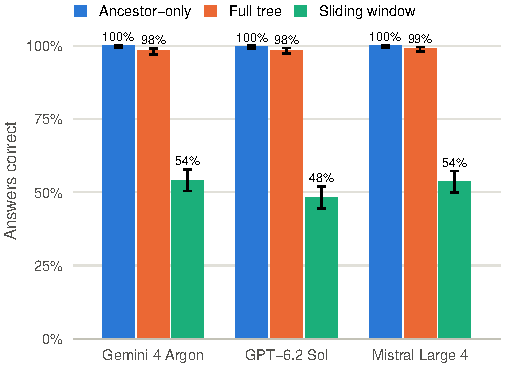
\includegraphics[width=0.75\textwidth]{fig4_correctness.pdf}
\end{center}

\textbf{What it shows.} The share of correct answers (judged measure) for each model and condition. About 720 answers per bar.

\begin{example}
\begin{center}
\small
\begin{tabular}{@{}lrrr@{}}
\toprule
Model & Ancestor & Full tree & Window \\
\midrule
Gemini 4 Argon & 100.0\% & 98.3\% & 54.2\% \\
GPT-6.2 Sol & 99.7\% & 98.5\% & 48.2\% \\
Mistral Large 4 & 100.0\% & 99.0\% & 53.6\% \\
\midrule
All three & 99.9\% & 98.6\% & 52.0\% \\
\bottomrule
\end{tabular}
\end{center}
\end{example}

\textbf{How to read it.} The pattern is the same for every model: ancestor-only and full tree near the top, the window around half. So the finding is about the rules, not one model.

\textbf{In one sentence:} every model answered almost perfectly with ancestor-only or the full tree, and about half the time with an equal-size window.

\section{Quality scores}

\begin{center}
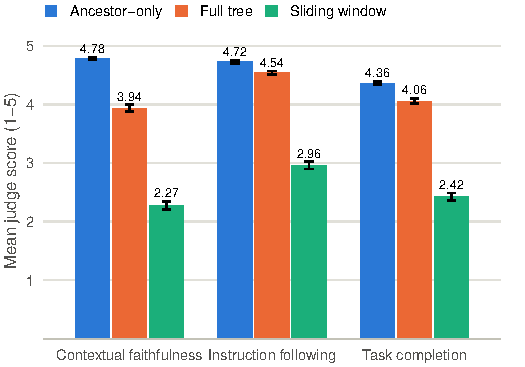
\includegraphics[width=0.75\textwidth]{fig5_quality.pdf}
\end{center}

\textbf{What it shows.} Average judge scores (1 to 5) for each criterion and condition, about 2,160 answers per bar. The paper reports these in Table III.

\begin{example}
\begin{center}
\small
\begin{tabular}{@{}lrrr@{}}
\toprule
Criterion & Ancestor & Full tree & Window \\
\midrule
Contextual faithfulness & 4.78 & 3.94 & 2.27 \\
Instruction following & 4.72 & 4.54 & 2.96 \\
Task completion & 4.36 & 4.06 & 2.42 \\
\bottomrule
\end{tabular}
\end{center}
Paired differences from ancestor-only, with bootstrap intervals: full tree faithfulness $-0.85$ ($-0.92$ to $-0.78$); window faithfulness $-2.51$ ($-2.63$ to $-2.39$). All Holm-adjusted $p < 10^{-6}$.
\end{example}

\textbf{How to read it.} Ancestor-only is highest on every criterion. The full tree loses most on faithfulness: it is usually correct but often brings in details or alternatives that are not part of the conversation being continued. The window loses heavily on everything.

\textbf{In one sentence:} ancestor-only gave the best answers on every quality measure; the full tree was correct but less faithful, and the window was worse on everything.

\section{What the window loses (paper Fig.~6)}

\begin{center}
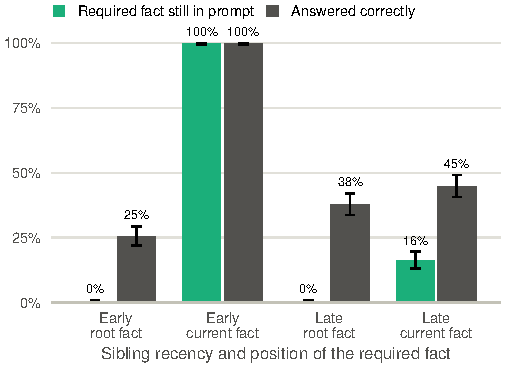
\includegraphics[width=0.75\textwidth]{fig6_window_displacement.pdf}
\end{center}

\textbf{What it shows.} Window answers only, split into the four combinations of sibling recency and fact position. Green bars: the share of prompts that still contained the required fact. Grey bars: the share of answers correct. About 540 answers per group.

\begin{example}
\begin{center}
\small
\begin{tabular}{@{}lrr@{}}
\toprule
Situation & Fact still in prompt & Correct \\
\midrule
Early siblings, fact near root & 0\% & 25.4\% \\
Early siblings, fact near current turn & 100\% & 100.0\% \\
Late siblings, fact near root & 0\% & 37.8\% \\
Late siblings, fact near current turn & 16.1\% & 44.8\% \\
\bottomrule
\end{tabular}
\end{center}
When the fact was still in the window, answers were correct 99.8\% of the time; when it had been pushed out, 32.4\%.
\end{example}

\textbf{How to read it with the formulas.}
\begin{itemize}
\item \textbf{Root, either recency:} 0\% kept. Proposition 5: the root is never in the window when siblings exist.
\item \textbf{Early siblings, current-turn fact:} 100\% kept. The fact is in the newest messages, after the siblings, so the window reaches it first.
\item \textbf{Late siblings, current-turn fact:} 16.1\% kept. The siblings are the newest messages and fill the window first; the fact survives only when the siblings are small (Proposition 6).
\item Answers can still be correct without the fact, mostly when a consistent sibling repeated the right value, or by a lucky guess.
\end{itemize}

\textbf{In one sentence:} the window's errors are almost entirely explained by whether it kept the required fact, exactly as the formulas predict.

\section{The price of ancestor-only (paper Fig.~7)}

\begin{center}
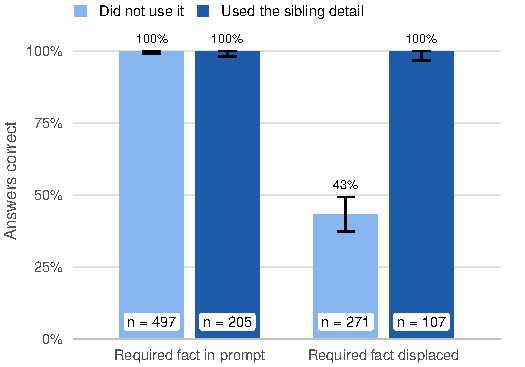
\includegraphics[width=0.75\textwidth]{fig7_consistent_price.pdf}
\end{center}

\textbf{What it shows.} Only answers with a consistent sibling, in the full tree and window. They are split by whether the required fact was still in the prompt (left pair versus right pair) and by whether the answer used the sibling's detail (light versus dark bar). The ``n ='' labels give the number of answers.

\begin{example}
Fact in prompt: 100\% correct whether or not the detail was used. Fact displaced: 43.2\% correct when the detail was not used (271 answers), 100\% when it was (107 answers). Fisher's exact test: $p < 10^{-30}$.
\end{example}

\textbf{What it means.} A consistent sibling restates the correct value (``If we stick with cuid2 keys \dots''). When the window has lost the original decision, that repetition is the only place the model can find the right answer, and using it rescues correctness. This is the one situation where sibling content helps.

\textbf{But:} the judge scored those same answers lower on faithfulness ($-1.28$ points) and task completion ($-0.36$), because they present details that are not in the active path as agreed.

\begin{ask}
\textbf{``So ancestor-only does lose something?''}\par
In principle, yes: a consistent sibling can hold useful information that ancestor-only never sends. In this experiment that only helped when a window had \emph{already} lost the required fact, and under ancestor-only the required fact is always present, so ancestor-only never lost an answer because of it. In real use, a side branch might contain a useful fact that was never stated on the main line; that is the case where combining the active path with retrieval from siblings would help, and it is the paper's suggested future work.
\end{ask}

\section{Robustness: do the results repeat?}

The 73 scenarios run three times show how stable each outcome is. The leakage outcome was identical across all three runs in 91.8\% to 100\% of cases, and correctness in 91.8\% to 100\%, depending on model and condition. Gemini's leakage was fully repeatable, and its correctness changed in a single full-tree scenario. Mistral varied most, consistent with deviation D1.

\textbf{In one sentence:} the results are stable from run to run; the conclusions do not depend on one lucky draw.
